\appendix

\chapter{Repositorio de código}
\label{anexo:repositorio}

\section{Ubicación del repositorio}
El código de este proyecto se encuentra disponible públicamente en el
siguiente repositorio:
\url{https://uvaes.sharepoint.com/:f:/r/sites/GRP-GestionEscuela-TFG/Documentos%20compartidos/TFG/RepositorioTFG/curso.2025.2026/daniel.gomez.arranz/doc.adicional?csf=1&web=1&e=568kT0}

\section{Organización del repositorio}
El código del repositorio se organiza en las siguientes carpetas principales:
\begin{itemize}
    \item \texttt{Code/MVP/}: Contiene los scripts del pipeline activo: \texttt{main.py} (motor GraphRAG principal), \texttt{chunk\_extractor.py} (extracción jerárquica de PDF) y \texttt{document\_strategy\_agent.py} (agente de estrategia).
    \item \texttt{Code/MVP/Pliegos/}: Directorio de documentos PDF de entrada utilizados durante las pruebas.
    \item \texttt{Tex\_files/}: Código fuente \LaTeX{} de esta memoria, organizado por capítulos.
    \item \texttt{images/}: Diagramas, capturas e imágenes referenciadas en la memoria.
    \item \texttt{Archivos\_Soporte/}: Documentación de apoyo y registros de pruebas.
\end{itemize}

\section{Instrucciones de inicio rápido}
El archivo \texttt{README.md} del repositorio resume los pasos para poner en marcha el sistema:
\begin{enumerate}
    \item Clonar el repositorio y acceder a \texttt{Code/MVP/}.
    \item Crear un entorno virtual e instalar dependencias con \texttt{pip install -r requirements.txt}.
    \item Asegurarse de que \texttt{Ollama} esté en ejecución y de que el modelo \texttt{llama3.1:8b} esté descargado (\texttt{ollama pull llama3.1:8b}).
    \item Colocar los PDFs a analizar en \texttt{Code/MVP/Pliegos/}.
    \item Ejecutar \texttt{python main.py} para iniciar la sesión de consulta interactiva.
\end{enumerate}
Para instrucciones detalladas, requisitos de hardware y resolución de problemas, véase el Apéndice~\ref{ape:manual}.

\chapter{Planificación Detallada por Incrementos}
\label{anexo:planificacion}

En este anexo se desglosa la planificación y los resultados de cada uno de los incrementos de desarrollo descritos en la sección de metodología. Cada tabla detalla las tareas técnicas específicas abordadas, los requisitos funcionales (RF) y no funcionales (RNF) asociados a cada una, y los entregables o resultados concretos obtenidos al finalizar cada tarea.

\newpage
\section*{Incremento 1: MVP - Núcleo de Ingesta y RAG Básico (Semanas 8-9)}
El objetivo de este primer ciclo fue construir y validar un Producto Mínimo Viable (MVP) que demostrara la viabilidad del pipeline completo, desde la carga de un documento hasta la generación de una respuesta básica.

\begin{table}[H]
    \centering
    \renewcommand{\arraystretch}{1.3}
    \caption{Tareas detalladas y resultados del Incremento 1.}
    \label{tab:incremento1_detallado}
    \begin{tabularx}{\textwidth}{|X|c|X|}
    \hline
    \textbf{Tarea / Historia de Usuario} & \textbf{Requisitos Asociados} & \textbf{Entregable / Resultado} \\
    \hline
    \textbf{Desarrollar la carga de PDFs:} Implementar la lectura de archivos PDF utilizando la librería \texttt{PyMuPDF} y la extracción inicial de texto. & RF-01 & Script \texttt{chunk\_extractor.py} con funcionalidad básica de lectura de documentos. \\
    \hline
    \textbf{Implementar el chunking jerárquico:} Desarrollar la lógica de detección de TOC (hipervínculos y regex) y la inferencia de jerarquía (numérica y posicional) para segmentar el documento. & RF-02, RF-03, RF-04 & Funciones de detección de TOC y segmentación estructural implementadas y validadas, capaces de generar chunks con metadatos de nivel y parentalidad. \\
    \hline
    \textbf{Crear embeddings y búsqueda vectorial:} Integrar la librería \texttt{SentenceTransformer} para generar embeddings duales (título y contenido) y desarrollar una función para la búsqueda por similitud de coseno. & RF-07 & Módulo de embeddings funcional y una función de búsqueda vectorial que devuelve los chunks más relevantes para una consulta dada. \\
    \hline
    \textbf{Establecer la conexión con el LLM local:} Construir un prompt simple con el contexto recuperado y utilizar \texttt{Ollama} para generar una respuesta, validando el pipeline completo. & - & Pipeline de RAG básico de principio a fin, validando la conexión y la generación de respuestas a partir de un único documento. \\
    \hline
    \end{tabularx}
\end{table}

\newpage
\section*{Incremento 2: Sofisticación del RAG y Grafo (Semanas 10-11)}
En esta fase se transformó el pipeline RAG básico en un sistema avanzado de GraphRAG, implementando la representación del conocimiento en grafos y mejorando drásticamente la calidad de la recuperación de información.

\begin{table}[H]
    \centering
    \renewcommand{\arraystretch}{1.3}
    \caption{Tareas detalladas y resultados del Incremento 2.}
    \label{tab:incremento2_detallado}
    \begin{tabularx}{\textwidth}{|X|c|X|}
    \hline
    \textbf{Tarea / Historia de Usuario} & \textbf{Requisitos Asociados} & \textbf{Entregable / Resultado} \\
    \hline
    \textbf{Crear la clase base para el grafo:} Definir la estructura de nodos en \texttt{NetworkX} para almacenar metadatos (título, nivel, texto) y crear aristas jerárquicas y secuenciales. & RF-05 & Clase \texttt{NetworkXRAG} funcional, capaz de construir un grafo estructural a partir de los chunks de un documento. \\
    \hline
    \textbf{Implementar el enriquecimiento semántico:} Desarrollar la función \texttt{add\_semantic\_edges} que calcula la similitud de coseno entre todos los nodos no conectados y añade aristas si superan un umbral. & RF-06 & Grafo enriquecido que conecta conceptos relacionados a través de diferentes ramas jerárquicas del documento. \\
    \hline
    \textbf{Desarrollar la búsqueda híbrida:} Integrar la librería \texttt{rank\_bm25} y combinar sus puntuaciones con las de la búsqueda vectorial. Implementar el re-ranking de resultados con un modelo Cross-Encoder. & RF-10 & Función \texttt{query\_chunks\_hybrid} robusta que devuelve una lista de chunks iniciales con una alta precisión de relevancia. \\
    \hline
    \textbf{Diseñar el algoritmo de selección de contexto:} Implementar la lógica de \texttt{get\_optimal\_context} para calcular scores combinados (propagación familiar) y ponderarlos con métricas de centralidad del grafo. & RF-11 & Mecanismo de selección de contexto finalizado, que elige los nodos más informativos del grafo para responder a la consulta. \\
    \hline
    \end{tabularx}
\end{table}

\newpage
\section*{Incremento 3: Inteligencia de Agentes y Consolidación (Semana 12)}
El último incremento se centró en añadir una capa de inteligencia al sistema mediante agentes LLM y en escalar la solución para gestionar múltiples documentos y generar respuestas consolidadas.

\begin{table}[H]
    \centering
    \renewcommand{\arraystretch}{1.3}
    \caption{Tareas detalladas y resultados del Incremento 3.}
    \label{tab:incremento3_detallado}
    \begin{tabularx}{\textwidth}{|X|c|X|}
    \hline
    \textbf{Tarea / Historia de Usuario} & \textbf{Requisitos Asociados} & \textbf{Entregable / Resultado} \\
    \hline
    \textbf{Implementar el agente de optimización de consultas:} Crear el prompt y la lógica de la función \texttt{generate\_optimized\_query} para que un LLM refine la entrada del usuario, extrayendo los términos clave. & RF-09 & Agente de optimización funcional que mejora la eficacia de la búsqueda al enfocarla en los conceptos más relevantes de la pregunta. \\
    \hline
    \textbf{Desarrollar el agente de selección de estrategia:} Diseñar e implementar la clase \texttt{DocumentStrategyAgent} que, mediante un LLM, determina de forma autónoma si se debe usar RAG o el documento completo. & RF-08 & Agente de decisión integrado que permite al sistema adaptarse dinámicamente al tipo de consulta del usuario. \\
    \hline
    \textbf{Orquestar el flujo multi-documento:} Crear la clase \texttt{SmartDocumentProcessor} para integrar los agentes y desarrollar los modos de respuesta individual y consolidado. & RF-12 & Sistema completo capaz de manejar múltiples documentos, orquestar las decisiones de los agentes y sintetizar información de diversas fuentes. \\
    \hline
    \textbf{Añadir la capacidad de visualización del grafo:} Desarrollar la función \texttt{visualize\_query\_graph} para generar una imagen \texttt{.png} del subgrafo de consulta, facilitando la depuración y el análisis. & RNF-04 & Herramienta de trazabilidad visual que permite inspeccionar el razonamiento del sistema de GraphRAG. \\
    \hline
    \end{tabularx}
\end{table}

\chapter{Seguimiento del Proyecto con Kanban}
\label{anexo:kanban}

Para la gestión de las tareas durante las fases de desarrollo, se utilizó un tablero Kanban en la herramienta Trello. Este anexo documenta visualmente el progreso del proyecto al finalizar cada uno de los tres incrementos de desarrollo.
\newpage
\section*{Estado del Tablero al Finalizar el Incremento 1}
La Figura \ref{fig:kanban_inc1} muestra el estado del tablero tras completar las tareas del primer incremento (MVP). Se puede observar cómo las funcionalidades básicas de ingesta y RAG simple han sido movidas a la columna \textit{Finalizado (Done)}, mientras que las tareas de los siguientes incrementos permanecen en \textit{Pendiente (To Do)}.

\begin{figure}[H]
    \centering
    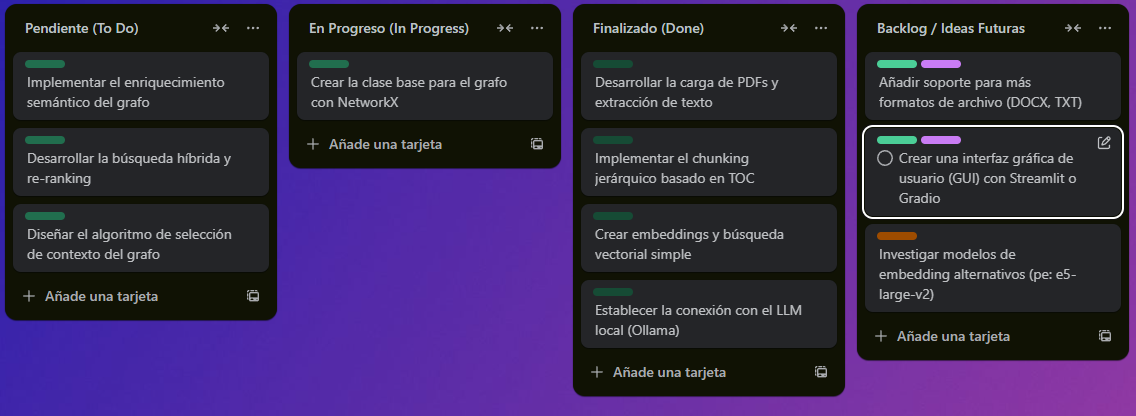
\includegraphics[width=0.9\textwidth]{images/kanban_fin_incremento1.png} % Cambia esto a la ruta de tu imagen
    \caption{Captura del tablero Kanban al finalizar el Incremento 1 (Semana 9).}
    \label{fig:kanban_inc1}
\end{figure}
\newpage
\section*{Estado del Tablero al Finalizar el Incremento 2}
Tras la finalización del segundo incremento, el tablero (Figura \ref{fig:kanban_inc2}) refleja la implementación de las funcionalidades de GraphRAG. Las tareas relacionadas con la creación de grafos y la búsqueda híbrida se encuentran ahora completadas. Las tareas del último incremento, centradas en los agentes, están a punto de comenzar.

\begin{figure}[H]
    \centering
    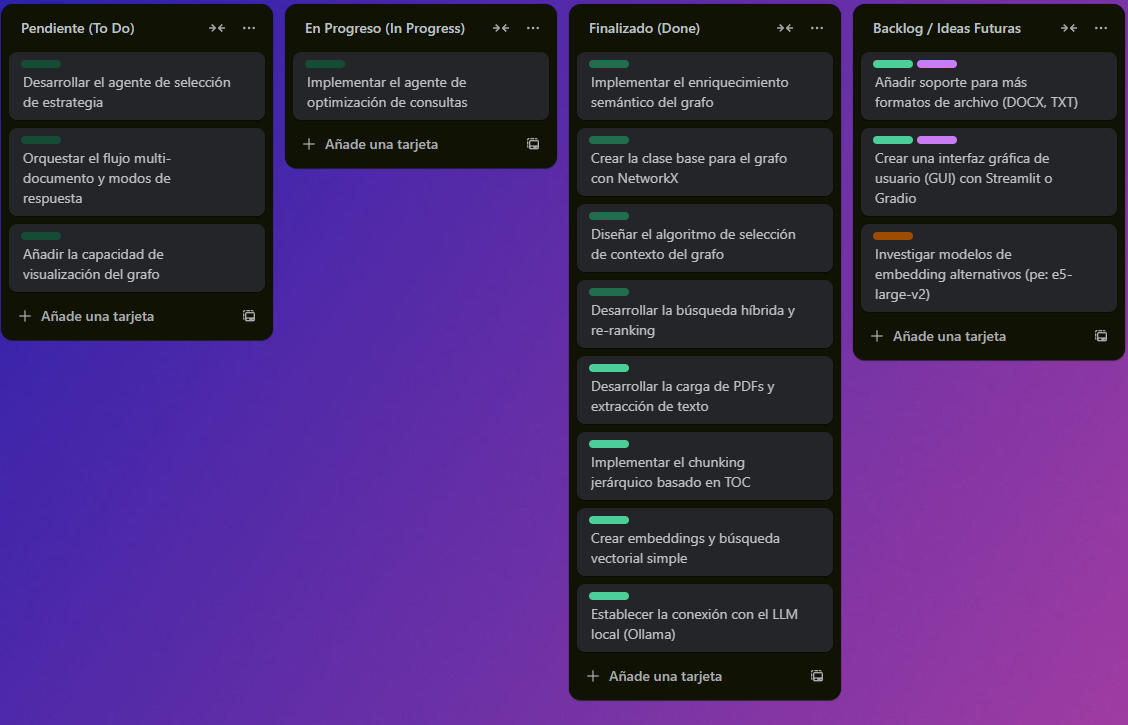
\includegraphics[width=0.9\textwidth]{images/kanban_fin_incremento2.png} % Cambia esto a la ruta de tu imagen
    \caption{Captura del tablero Kanban al finalizar el Incremento 2 (Semana 11).}
    \label{fig:kanban_inc2}
\end{figure}
\newpage
\section*{Estado del Tablero al Finalizar el Incremento 3}
La Figura \ref{fig:kanban_inc3} presenta el estado final del tablero una vez completado todo el desarrollo de software. Todas las tareas de implementación, incluyendo la integración de los agentes inteligentes y la gestión de múltiples documentos, han sido movidas a la columna \textit{Finalizado (Done)}, marcando la conclusión exitosa de la fase de desarrollo.

\begin{figure}[H]
    \centering
    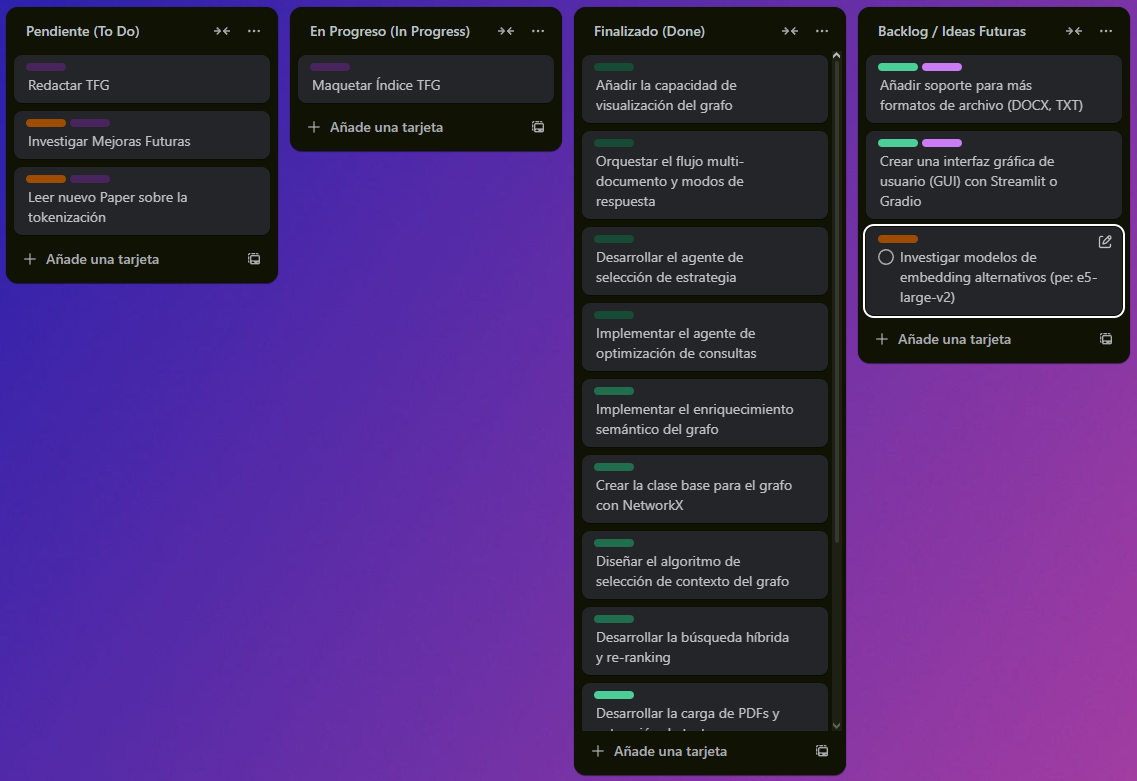
\includegraphics[width=0.9\textwidth]{images/kanban_fin_incremento3.png} % Cambia esto a la ruta de tu imagen
    \caption{Captura del tablero Kanban al finalizar la fase de implementación (Semana 12).}
    \label{fig:kanban_inc3}
\end{figure}